\documentclass{article}

\usepackage[margin=1in]{geometry}
\usepackage{tabularx}
\usepackage{amsmath}
\usepackage{tikz}

% Command for styling the boxes containing assignment instructions
\newcommand{\requirement}[1]{\noindent\fbox{\begin{minipage}{0.9\textwidth}
    \paragraph{Instructions}
    #1
\end{minipage} }}

\title{AI Powered Phishing Email Detection System}

\author{Mr. Rueben van der Westhuizen \\ u21434809}

\begin{document}

\maketitle
\newpage
\tableofcontents
\newpage

\section{Research Overview}

\subsection{How does AI detect Phishing attacks:}

AI is increasingly used to detect phishing attacks by analyzing various email characteristics such as sender behavior, message content, and embedded URLs to identify anomalies or patterns indicative of phishing attempts \cite{basit2021comprehensive}. Machine learning algorithms, including natural language processing (NLP) and deep learning, are employed to recognize subtle cues that traditional rule  based systems might miss \cite{Wang2020Feature} \cite{Lauriola2021An}. ML algorithms, especially classifiers like Logistic Regression, Random Forests, and Neural Networks, are trained to identify patterns in email content, metadata, and even the tone of the language used can continuously learn from new data, improving their detection accuracy over time without manual updates \cite{Karim2019A} \cite{Murti2023Machine}.

\subsection{Traditional methods}

Compared to traditional methods, AI can handle large volumes of email traffic and detect novel, previously unseen phishing tactics. Its ability to adapt to new attack strategies makes it more effective in protection that is real time \cite{Jalil2022Highly} \cite{Alsariera2020AI} \cite{Basit2020A}.

\subsection{Advantages}
AI powered phishing detection is also less prone to false positives, ensuring legitimate emails are not mistakenly flagged. Additionally, AI systems can automate responses, reducing the need for manual intervention \cite{Basit2020A}. This leads to faster threat mitigation and enhanced user security \cite{Sameen2020PhishHaven—An}. By integrating AI, organizations can build a more robust defense against the evolving landscape of phishing threats \cite{Kumar2024What} \cite{Chinnasamy2024AI}.


\newpage

\section{Model selection process}
Selection of Kaggle's Phishing Email Dataset:
After close inspection, a combination off the "CEAS 08.csv" dataset, "NigerianFraud.csv", "SpamAssasin.csv", and "Nazario.csv" from has approximately 48,762 emails sum total after cleaning. 

\subsection{Data Preprocessing and Feature Extraction }

\begin{itemize}
    \item Subject: Has sufficient data without any missing values 
    \item Body: Has sufficient data without any missing values
    \item label (Spam or legitimate)
\end{itemize}


\subsection{Machine Learning Models Considered}
\begin{itemize}
    \item Logistic Regression
    \item Random Forest
    \item Neural Networks
\end{itemize}

\subsection{Model Selection Justification}
The model selection process for phishing email detection begins with evaluating the type of data available (email content, sender information, subject line, etc.) and the complexity of the task. Given that phishing emails often contain subtle cues, we need models that can identify these implied meaning in unstructured (text) data.

Initially, simpler models like Logistic Regression (LR) and Random Forest (RF) are considered. LR serves as a baseline because of its simplicity and interpretability, making it easier to understand which features are influencing the predictions. However, it may struggle with capturing nonlinear relationships and complex interactions between features.

On the other hand, Random Forest is an ensemble method that performs better on diverse datasets because it combines multiple decision trees, which helps in reducing overfitting. It is also able to capture nonlinear relationships in the data, making it more robust than LR.

For more complex patterns in the data, we consider Neural Networks (NN). Specifically, Multilayer Perceptrons (MLPs) or Recurrent Neural Networks (RNNs) are employed for text data, as they excel at recognizing sequential patterns in the email content, such as unusual phrasing or tone that might signal phishing. Additionally, long-short-term memory (LSTM) networks are considered for their ability to learn from sequences, making them highly effective for analyzing email texts with contextual meaning.

Model performance using metrics such as Accuracy, Precision, Recall, and F1-Score is crucial in evaluating phishing email detection systems. While Random Forest and Neural Networks typically offer the best results in terms of recall (catching phishing emails), Neural Networks—especially those with deep learning layers—tend to perform exceptionally well in detecting subtle, unseen phishing tactics. However, these models generally require longer training times, especially deep learning models, due to the complexity and the large amount of data they process during training.

Ultimately, Random Forest was selected for its balance between performance and interoperability and also provide feature importance scores.

\[
\begin{array}{|c|c|c|c|c|c|}
\hline
\textbf{Model} & \textbf{Accuracy (\%)} & \textbf{Precision (\%)} & \textbf{Recall (\%)} & \textbf{F1-Score (\%)} & \textbf{Notes} \\
\hline
\text{Logistic Regression} & 98.08 & 97.88 & 98.50 & 98.19 & \text{Simple, interpretable, fast} \\
\text{Random Forest} & 98.02 & 97.52 & 97.87 & 97.69 & \text{Handles non-linear data well} \\
\text{Neural Networks} & 99.40 & 98.70 & 99.00 & 98.80 & \text{Captures complex patterns} \\
\hline
\end{array}
\]
\newpage


\section{Requirements Specification}

The AI Powered Phishing Email Detection System is designed as a full stack web application that enables users to submit email content and receive real time predictions on whether the email is phishing or legitimate. The system leverages a machine learning backend and a user friendly frontend to provide accurate, fast, and interpretable results.

\subsection{Functional Requirements}
\begin{itemize}
    \item Users can submit email text (subject and body) via a web interface.
    \item The system processes the input and returns a prediction (phishing/legitimate) with a confidence score.
    \item The backend exposes a REST API endpoint for predictions.
    \item The frontend displays results, highlights suspicious words, and visualizes confidence.
    \item The system supports retraining and updating the ML model with new data.
\end{itemize}

\subsection{Non-Functional Requirements}
\begin{itemize}
    \item The system must respond to prediction requests within 2 seconds.
    \item The model must achieve at least 97\% accuracy on the test set.
    \item The web interface must be accessible and responsive on desktop and mobile devices.
    \item The backend and frontend must be easily deployable on standard Windows or Linux environments.
    \item Security: Only sanitized input is processed; no user data is stored.
\end{itemize}

\subsection{System Components}
\begin{itemize}
    \item \textbf{Frontend:} Angular SPA for user interaction.
    \item \textbf{Backend:} Flask REST API for ML inference.
    \item \textbf{ML Model:} Trained Random Forest, serialized as \texttt{model.pkl}.
    \item \textbf{Data:} Preprocessed datasets from multiple sources (CEAS, NigerianFraud, SpamAssassin, Nazario).
\end{itemize}
\newpage
\subsection{UML Diagrams} 
\begin{itemize}
    \item \textbf{System Architecture:} Shows the interaction between frontend, backend, and model.
    % Insert system architecture image
    \begin{figure}[h!]
        \centering
        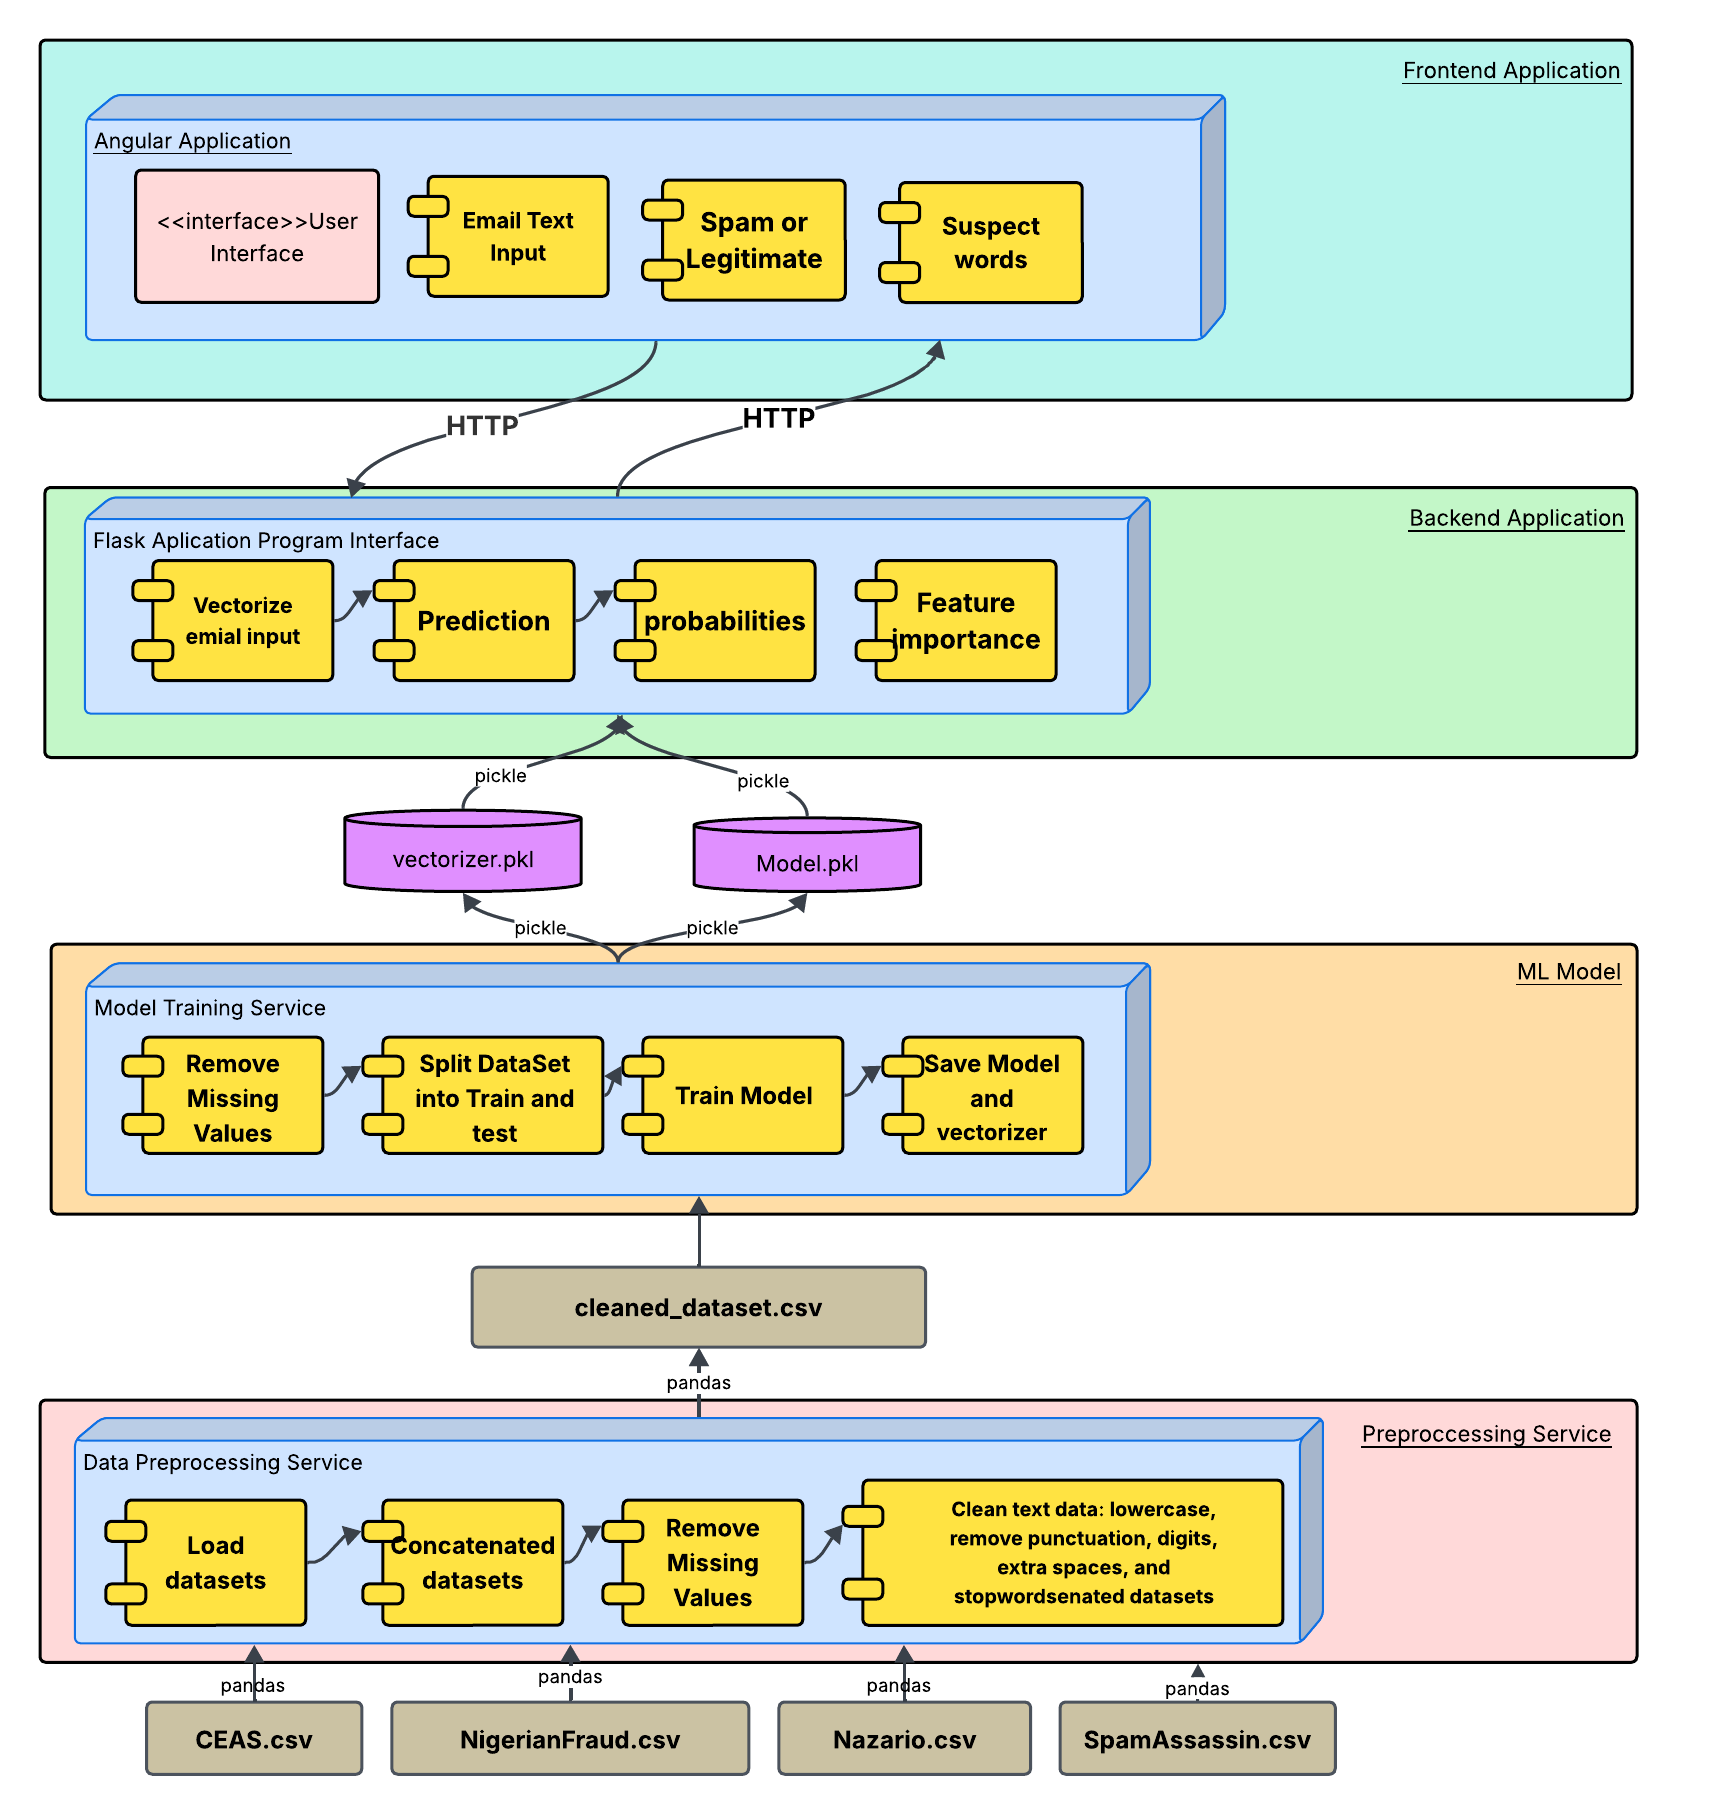
\includegraphics[width=0.8\textwidth]{Architecture.png}
        \caption{System Architecture of the AI Powered Phishing Email Detection System}
        \label{fig:system-architecture}
    \end{figure}

    \newpage
    \item \textbf{Workflow:} Sequence of user input, API call, prediction, and result display.
    % Insert system Sequence Diagrams image
    \begin{figure}[h!]
        \centering
        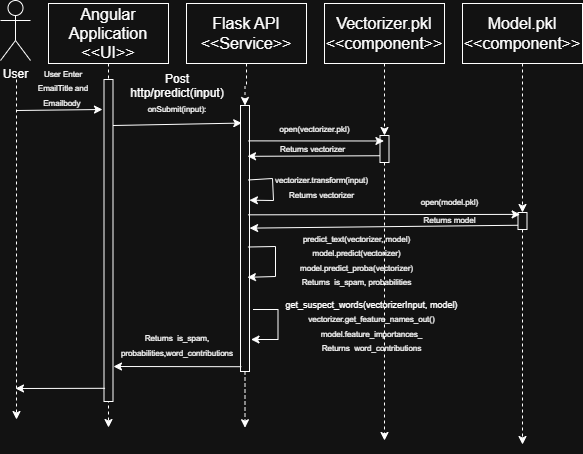
\includegraphics[width=0.8\textwidth]{Sequence.png}
        \caption{Workflow of the AI Powered Phishing Email Detection System}
        \label{fig:workflow}
    \end{figure}
    

\end{itemize}



\section{Conclusion and Future Work}

\subsection{Summary of Findings}

\subsection{Potential Enhancements}

\newpage

\bibliographystyle{bibstyle}
\bibliography{sources}

\end{document}
